\documentclass[conference]{IEEEtran}
\IEEEoverridecommandlockouts
\usepackage{cite}
\usepackage{amsmath,amssymb}
\usepackage{graphicx}
\usepackage{booktabs}
\usepackage{algorithm}
\usepackage{algpseudocode}
\usepackage{textcomp}
\usepackage{xcolor}
\usepackage{tikz}
\usetikzlibrary{positioning,fit,arrows.meta,calc}
\usepackage{array}
\usepackage{url}
\usepackage[hidelinks]{hyperref}

\newcommand{\us}{\,\textmu s}
\newcommand{\ms}{\,ms}
\newcommand{\cpuweight}{\texttt{cpu.weight}}

\begin{document}

\title{eBPF-Based Detection and Mitigation of CPU Scheduling Unfairness Under Mixed Workloads}

% Four names side by side, one shared affiliation line underneath.
\author{%
\IEEEauthorblockN{\begin{tabular}{@{}c@{\hspace{1.2em}}c@{\hspace{1.2em}}c@{\hspace{1.2em}}c@{}}
Gokul Krishna Balaji & Garikina Asish Preetam & Bhyrapuneni Venkat Manoj & Karra Sunith Vardhan Singh\\
\normalsize CS24B2053 & \normalsize CS24I1022 & \normalsize CS24B2052 & \normalsize CS24B2017
\end{tabular}}
\IEEEauthorblockA{Indian Institute of Information Technology, Design and Manufacturing, Kancheepuram}}

\maketitle

\begin{abstract}
Latency-sensitive tasks that share CPUs with batch work suffer tail-latency inflation that long-run CPU-share metrics do not reveal. We build an eBPF collector that records, for every thread, how long it waits runnable on the run queue. We validate it against kernel trace events (706 of 706 waits matched, median difference 0.12\us) and against the kernel's own accounting (aggregate difference 0.02\%), then use it to characterize Linux's EEVDF scheduler and to drive \emph{WaitBoost}, a bounded, aging and starvation-guarded boost that runs in user space and needs neither application nor kernel changes. Across 270 paired runs on Linux 6.18 with three interactive mixes and one to four batch threads per core, EEVDF inflates interactive p99 response time 1.7--4.0$\times$ over running alone and misses the latency objective for up to 20\% of requests, while Jain's index over normalized CPU shares stays above 0.95. Our central finding is that when the two classes run in separate cgroups, the default under systemd and container runtimes, per-task knobs cannot move CPU time between them: static nice, a static EEVDF custom slice and WaitBoost driving either knob leave p99 unchanged or worse. Class-level weight works: a static 4:1 \cpuweight{} cuts p99 by 42\% (all 45 seed pairs improve) with batch throughput within 2\%, and by 39--46\% on a held-out mix, while WaitBoost driving that knob cuts p99 by 14\%. The collector costs about 0.55\us{} per scheduler event.
\end{abstract}

\begin{IEEEkeywords}
eBPF, CPU scheduling, EEVDF, fairness, tail latency, cgroups
\end{IEEEkeywords}

% ===================================================================================== I
\section{Introduction}

\subsection{Background}
Multiplexing many runnable tasks over a few cores is the basic job of an operating-system scheduler, and the task mix is rarely uniform. Request handlers and media pipelines sleep most of the time and need the CPU briefly but promptly, while compilers and analytics jobs would use every cycle they are given. A general-purpose scheduler must keep throughput high, give every task its fair share, and still let a freshly woken interactive task run quickly. Since version 6.6, Linux pursues these goals with EEVDF (Earliest Eligible Virtual Deadline First)~\cite{stoica1996eevdf,kernel-eevdf}, which replaced CFS. EEVDF tracks each task's \emph{lag} against an ideal fluid share and, among the tasks that are owed CPU time, runs the one with the earliest virtual deadline. Since Linux 6.12 a task may also request a shorter time slice, which gives it earlier deadlines~\cite{corbet2024eevdf}. eBPF~\cite{kernel-bpf} lets us watch these decisions on an unmodified kernel by attaching verified programs to scheduler tracepoints.

\subsection{Problem Definition}
Let $I$ be a set of interactive tasks and $B$ a set of batch tasks sharing $k$ cores. Interactive requests arrive open-loop: request $j$ arrives at time $a_j$ regardless of earlier requests and completes at $e_j$, so its response time
\begin{equation}
R_j = e_j - a_j
\end{equation}
includes every interval in which the request's thread was runnable but not running, its \emph{run-queue wait}. Batch tasks are CPU-bound and are measured in completed work units per second. The schedule is unfair to the interactive class when batch contention inflates the tail of $R$. We quantify this by the slowdown $S = P_{99}(R \mid B) / P_{99}(R \mid \emptyset)$, by the fraction of requests that miss a service-level objective (SLO), and by \emph{unfairness episodes}, maximal runs of consecutive 100\ms{} windows whose worst response time exceeds the SLO. Unfairness to the batch class is measured by the normalized share $n_i = c_i / f_i$, where $c_i$ is the CPU time task $i$ received and $f_i$ its max-min fair entitlement given its demand, summarized over all $N$ tasks by Jain's index~\cite{jain1984fairness}
\begin{equation}
J = \frac{\left(\sum_i n_i\right)^2}{N \sum_i n_i^2},
\end{equation}
and by starvation: the longest run-queue wait of any batch thread and the number of 100\ms{} windows in which a batch thread completed no work. The problem is to detect such unfairness with low-overhead kernel telemetry and to reduce interactive tail latency while losing at most 5\% of batch throughput and never starving batch work. We test three hypotheses. \textbf{H1}: under EEVDF, batch contention inflates interactive p99 by more than 1.5$\times$ and produces multi-window episodes even when long-run shares are fair. \textbf{H2}: a lightweight policy driven by eBPF-measured run-queue wait reduces interactive p99 within the throughput and starvation limits. \textbf{H3}: acting through the EEVDF slice matches the p99 benefit of acting through weight while disturbing CPU shares less, because a slice changes \emph{when} a task runs rather than \emph{how much} CPU it receives.

\subsection{Objectives and Contributions}
Our objectives are to (O1) measure run-queue unfairness accurately and cheaply, (O2) mitigate it with mechanisms available in a stock kernel, and (O3) evaluate the outcome rigorously for both classes. We contribute:
\begin{itemize}
\item \textbf{C1}: a validated eBPF collector of per-thread run-queue wait and a characterization of EEVDF on Linux 6.18 that confirms H1 (\S\ref{sec:h1}).
\item \textbf{C2}: \emph{WaitBoost}, an application-agnostic, bounded, aging and starvation-guarded boost driven by per-thread wait sampled every 10\ms, with three actuators: nice, the EEVDF custom slice and cgroup \cpuweight{} (\S\ref{sec:waitboost}).
\item \textbf{C3}: the finding that per-task actuators are inert across cgroup boundaries, so only class-level weight cuts tail latency, by 42\%, at no measurable throughput cost. H3 is rejected (\S\ref{sec:mitigation}).
\item \textbf{C4}: a paired-seed evaluation with bootstrap confidence intervals, ablations, a held-out mix, and overhead and scaling runs, packaged as a reproducible artifact.
\end{itemize}

% ===================================================================================== II
\section{Literature Survey and Research Gaps}

\textit{Characterizing Linux scheduling.} Lozi et al.~\cite{lozi2016wasted} showed that load-balancing bugs in CFS left runnable threads waiting while cores sat idle, a problem that went unnoticed for years until targeted tracing exposed it. Bouron et al.~\cite{bouron2018battle} compared FreeBSD's ULE with CFS and found that ULE's interactivity heuristic can favour sleepy threads strongly enough to starve batch work. Li et al.~\cite{li2014tales} traced server tail latency to OS sources such as scheduling order, background tasks and interrupt placement, and removed them with static configuration such as dedicated cores and real-time priority. The closest ancestor of our study is Leverich and Kozyrakis~\cite{leverich2014reconciling}. They showed that co-located batch jobs inflate memcached's tail latency under CFS's wake-up handling, and they fixed it by adding borrowed-virtual-time scheduling to the kernel. All of these studies predate EEVDF.

\textit{Latency boosts and proportional share.} BVT~\cite{duda1999bvt} lets a latency-sensitive thread \emph{warp} its virtual time backwards by a bounded amount, which gives it dispatch preference without changing its long-run share. The warp parameters are static. EEVDF~\cite{stoica1996eevdf} adds eligibility and virtual deadlines to proportional share, and Linux's custom slices~\cite{corbet2024eevdf} expose a per-task deadline knob. We found no peer-reviewed evaluation of that knob as a latency actuator.

\textit{Co-location controllers.} Heracles~\cite{lo2015heracles} keeps a latency-critical service within its SLO by taking cores, cache ways, memory bandwidth and power away from best-effort jobs. It is driven by the service's own reported tail latency, in a loop measured in seconds. PARTIES~\cite{chen2019parties} extends the idea to several interactive services with a 500\ms{} loop. Caladan~\cite{fried2020caladan} reacts at microsecond timescales but needs a custom runtime, a dedicated scheduling core and a kernel module.

\textit{Programmable schedulers.} ghOSt~\cite{humphries2021ghost} delegates scheduling decisions to user-space agents through a new kernel scheduling class. Enoki~\cite{miller2024enoki} lets developers write kernel schedulers in safe Rust on a modified kernel. Skyloft~\cite{jia2024skyloft} schedules at microsecond granularity in user space using hardware user interrupts. Mainline Linux now accepts BPF schedulers through \texttt{sched\_ext}~\cite{kernel-sched-ext}, but the kernel studied here is built without it.

\textit{Gaps.} From the four core works~\cite{leverich2014reconciling,duda1999bvt,lo2015heracles,humphries2021ghost} and the surrounding literature we derive four gaps.
\textbf{G1}: peer-reviewed characterizations of mixed-workload scheduling on Linux target CFS. EEVDF, the default since 2023, has not been studied for interactive tail latency, batch fairness and starvation together.
\textbf{G2}: closed-loop controllers rely on application-reported latency at second-scale periods, or on custom runtimes and dedicated cores. An application-agnostic kernel signal at millisecond scale has not been evaluated.
\textbf{G3}: bounded latency boosts (BVT, ghOSt policies, Enoki, Skyloft) require kernel changes or special hardware. Whether stock knobs (nice, the EEVDF slice, cgroup weight) can implement them is an open question.
\textbf{G4}: the batch side is usually reported only as throughput or CPU share, rarely with starvation bounds, wait distributions or confidence intervals.
Contributions C1--C4 address G1--G4 respectively.

% ===================================================================================== III
\section{Methodology Used}

\begin{figure}[t]
\centering
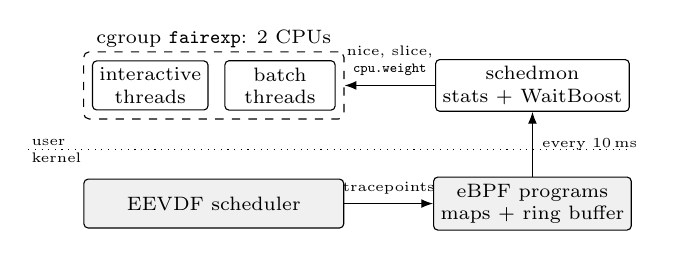
\begin{tikzpicture}[font=\scriptsize, >={Latex[length=1.5mm]},
  box/.style={draw, rounded corners=1.5pt, align=center, inner sep=2.5pt, minimum height=0.62cm},
  kbox/.style={box, fill=black!6}]
  \node[box, minimum width=1.4cm] (int) at (0,0) {interactive\\threads};
  \node[box, minimum width=1.4cm, right=0.2cm of int] (bat) {batch\\threads};
  \node[draw, dashed, rounded corners=2pt, fit=(int)(bat), inner sep=3pt,
        label={[font=\scriptsize, inner sep=1pt]above:cgroup \texttt{fairexp}: 2 CPUs}] (cg) {};
  \node[box, minimum width=2.1cm, right=1.15cm of cg] (sm) {schedmon\\stats + WaitBoost};
  \node[kbox, minimum width=3.3cm, below=0.75cm of cg] (sched) {EEVDF scheduler};
  \node[kbox, minimum width=2.1cm] (bpf) at (sched -| sm) {eBPF programs\\maps + ring buffer};
  \draw[->] (sm) -- node[above, font=\tiny, align=center]{nice, slice,\\\texttt{cpu.weight}} (cg);
  \draw[->] (sched) -- node[above, font=\tiny]{tracepoints} (bpf);
  \draw[->] (bpf) -- node[right, font=\tiny]{every 10\,ms} (sm);
  \coordinate (mid) at ($(cg.south)!0.5!(sched.north)$);
  \draw[dotted] (-1.55,0 |- mid) -- (sm.east |- mid);
  \node[anchor=south west, font=\tiny, inner sep=1pt] at (-1.55,0 |- mid) {user};
  \node[anchor=north west, font=\tiny, inner sep=1pt] at (-1.55,0 |- mid) {kernel};
\end{tikzpicture}
\caption{Experimental system. The two classes run in sibling cgroups on two CPUs; schedmon runs on a housekeeping CPU and closes the loop through stock kernel knobs.}
\label{fig:arch}
\end{figure}

\subsection{System Overview}
Fig.~\ref{fig:arch} shows the system. A workload generator runs the interactive and the batch threads as two processes placed in sibling cgroups, \texttt{fairexp/interactive} and \texttt{fairexp/batch}. Their parent cgroup confines both to $k=2$ experiment CPUs, and system services are confined to a separate housekeeping CPU. The collector, \emph{schedmon}, loads eBPF programs that update per-thread maps and a ring buffer. Its user-space half runs on a housekeeping CPU, dumps statistics, and optionally runs WaitBoost, writing nice values, slices or cgroup weights back to the kernel. A Python harness runs the experiments, and the analysis scripts compute every metric, table and figure in this paper from the raw run records. The implementation uses libbpf~\cite{libbpf} and bpftool~\cite{bpftool}, validation uses \texttt{trace-cmd}~\cite{tracecmd}, and the analysis uses NumPy~\cite{numpy}, SciPy~\cite{scipy}, pandas~\cite{pandas} and Matplotlib~\cite{matplotlib}.

\subsection{Workload Model}
Each interactive thread follows a precomputed, seeded schedule of arrival times and work amounts. It sleeps until the next arrival with an absolute-time \texttt{clock\_nanosleep} and then spins for a calibrated amount of work. A late request therefore never delays the next arrival, and response times are free of coordinated omission. \textbf{M1}: 2 threads, Poisson arrivals at 100/s each, 1\ms{} of work, SLO 5\ms. \textbf{M2}: 8 threads at 50/s, 0.5\ms{} of work, SLO 2.5\ms. \textbf{M3}: 4 threads with on/off bursts (400/s for 100\ms, then 400\ms{} idle), lognormal work with median 0.5\ms{} ($\sigma=0.5$), SLO 2.5\ms. The held-out mix \textbf{M4}, never used for tuning, models four 60\,Hz frame loops (16.7\ms{} period, $\pm$1\ms{} jitter, lognormal work with median 2\ms{} and $\sigma=0.6$) with the frame time as its SLO. Batch threads spin in 1\ms{} work units, and contention level x$k$ places $k$ batch threads on each experiment core. Together the interactive threads need about 9--10\% of the two cores in M1--M3 and 29\% in M4, so their class is demand-limited and its fair entitlement equals its demand. Each run has a 5\,s warm-up followed by a 30\,s measured window. Reference runs without batch work (x0) give the denominator of the slowdown.

\subsection{Telemetry and Validation}
schedmon attaches BTF-typed tracepoint programs to \texttt{sched\_wakeup} and \texttt{sched\_wakeup\_new}, which stamp the time a thread becomes runnable. A third program on \texttt{sched\_switch} closes the wait of the incoming thread and adds to the outgoing thread's run time. If the outgoing thread was preempted while still runnable, the program counts an involuntary switch and stamps it runnable again. A fourth program on \texttt{sched\_migrate\_task} counts migrations. Only threads whose cgroup is in a filter map are traced. A per-thread hash map holds the wait count, sum and maximum, a log$_2$ wait histogram, run time, voluntary and involuntary switches, and migrations. Every completed wait is also streamed through a ring buffer whose drop counter is reported. Each entry stores both the kernel thread id and the id local to the PID namespace (read with CO-RE), so records join with user-space logs inside containers and WSL.

We validate the collector against waits computed independently from a \texttt{trace-cmd} recording of all CPUs and against the kernel's \texttt{run\_delay} from \texttt{/proc/<tid>/schedstat}, which each thread reads when it exits. Its cost comes from the kernel's BPF runtime statistics and paired runs without the collector.

\subsection{WaitBoost}\label{sec:waitboost}
Every $\Delta=10$\ms, WaitBoost reads each traced thread's cumulative wait, run time and event count from the BPF map and updates three exponentially weighted moving averages ($\alpha=0.3$). They are the mean wait per scheduling event $\bar w$ (including any wait still in progress), the fraction of time asleep $\hat s$, and the fraction of time running $\hat c$. Like ULE's interactivity score, the test that a thread is latency-like needs no help from the application: $\hat s \ge 0.5$ and $\hat c \le C = 0.5$. Algorithm~\ref{alg:wb} maps these signals to a boost level $L \in \{0,\dots,3\}$. The \emph{guard} gives the maximum level to any thread, of either class, that has been runnable for $G=100$\ms{} without running. The \emph{revoke} rule bounds the boost to threads that stay light, and \emph{decay} ages a boost away after $D=50$\ms{} per level.

Three actuators translate $L$ into a stock kernel knob. \emph{nice} sets the thread's nice value to its original value minus $3L$, which raises its weight. \emph{slice} requests an EEVDF slice of $s_0/2^L$, where $s_0$ is the base slice. The slice is never shorter than 1.25 times the thread's typical CPU burst, so a boosted request is not cut mid-burst, and it stays within $[0.1\ms, s_0]$. \emph{cgweight} is a per-class variant. The interactive class's aggregate wait drives the interactive cgroup's \cpuweight{} to $100 \cdot 2^L$, and the boost is dropped whenever any batch thread has waited $G$. Every changed knob is restored on exit, and the harness verifies the restoration. The threshold $\theta$ was tuned on separate seeds (1--3) using M1 and M2 at x2. The rule was to take the lowest median p99 ratio among values of $\theta$ whose throughput ratio is at least 0.97. It selected $\theta=2$\ms{} for both per-thread actuators, and the parameters were frozen before any evaluation run. The cgroup variant uses the untuned default $\theta=0.5$\ms.

\begin{algorithm}[t]
\caption{WaitBoost decision for one thread per tick}
\label{alg:wb}
\footnotesize
\begin{algorithmic}[1]
\State update $\bar w, \hat s, \hat c$ from the map deltas since the last tick
\If{thread has been runnable for $\ge G$} \State $L \gets L_{\max}$ \Comment{starvation guard}
\ElsIf{$L>0$ \textbf{and} $\hat c > C$} \State $L \gets 0$ \Comment{revoke: no longer light}
\ElsIf{$\hat s \ge s_{\min}$ \textbf{and} $\hat c \le C$ \textbf{and} $\bar w > \theta$} \State $L \gets \min(L+1, L_{\max})$ \Comment{boost}
\ElsIf{$L>0$ \textbf{and} last change $\ge D$ ago} \State $L \gets L-1$ \Comment{aging}
\EndIf
\State apply actuator($L$); log the action
\end{algorithmic}
\end{algorithm}

\subsection{Baselines}
\textbf{B0} is stock EEVDF: every thread at nice 0 and equal cgroup weights. \textbf{B1} is a static priority with every batch thread at nice 10. \textbf{B2} is a static class weight, with the interactive cgroup at \cpuweight{} 400 and the batch cgroup at 100. \textbf{B3} is a static 0.3\ms{} EEVDF slice for every interactive thread. WB-nice and WB-slice are WaitBoost with the two per-thread actuators. WB-cg, the per-cgroup variant, appears among the ablations.

\subsection{Experimental Design and Statistics}
The main grid crosses three mixes, three contention levels, six policies and five evaluation seeds (101--105), for 270 runs plus 15 reference runs. The held-out M4 grid adds 90 runs, the ablations at x2 add 180, core scaling ($k=1,2,3$) adds 75, overhead adds 45 and tuning used 54. Run order is randomized within blocks. A run interrupted by the host (detected from its wall-clock duration only, never from its results) is deleted and re-run. Within each cell we report medians with 95\% bootstrap confidence intervals (10\,000 resamples~\cite{efron1993bootstrap}). Policies are compared through ratios to B0 paired by seed, so both runs see identical arrivals. With five pairs, a two-sided Wilcoxon signed-rank test cannot reach $p<0.05$ (its minimum is 0.0625), so we also pool the 45 main pairs of each policy. Table~\ref{tab:repro} lists the platform, a quad-core laptop running Ubuntu 26.04 under WSL2.

\begin{table}[t]
\centering
\footnotesize
\caption{Experimental platform (from sysinfo.json).}
\label{tab:repro}
\begin{tabular}{@{}lp{0.68\columnwidth}@{}}
\toprule
Distribution & Ubuntu 26.04.1 LTS \\
Kernel & 6.18.54.1-microsoft-standard-WSL2 \\
Virtualization & wsl (clocksource tsc) \\
CPU & 11th Gen Intel(R) Core(TM) i5-1155G7 @ 2.50GHz (8 vCPU) \\
Memory & 7.6 GiB \\
Storage & /dev/sdd       ext4 1007G  2.9G  953G   1% / \\
Kernel config & HZ=250, PREEMPT\\_DYNAMIC=y, SCHED\\_CLASS\\_EXT=n \\
Scheduler & EEVDF, base slice 2800000 ns, preempt=(none) voluntary full lazy \\
Compilers & gcc (Ubuntu 15.2.0-16ubuntu1) 15.2.0; Ubuntu clang version 21.1.8 (6ubuntu1) \\
BPF tooling & libbpf 1.6.3; bpftool v7.7.0; bpftrace v0.25.0 \\
Analysis & Python 3.14.4, numpy 2.3.5, pandas 2.3.3, scipy 1.16.3 \\
Spin calibration & 627.2 iterations/\textmu s \\
\bottomrule
\end{tabular}
\end{table}


% ===================================================================================== IV
\section{Experimental Results}

\subsection{Telemetry Validity and Cost}
All 706 waits found in an independent \texttt{trace-cmd} recording were matched by the collector, with a median absolute difference of 0.12\us, a p99 of 2.1\us{} and a maximum of 18\us. Against the kernel's \texttt{run\_delay} (Fig.~\ref{fig:validation}), the aggregate difference over the 2520 threads of the loaded runs is $-0.015\%$ for batch threads and $-0.31\%$ for interactive threads. The median per-thread error is 0.008\% and 0.77\% respectively. Threads of the idle reference runs carry a fixed 11--24\ms{} excess whose source we have not isolated. It is visible only because those threads barely wait, and those runs enter our metrics only through response times, which the generator measures itself. Table~\ref{tab:overhead} gives the cost. The programs take 485--598\,ns per scheduler event and at most 0.036\% of the experiment CPUs, and the ring buffer dropped none of the 6.7\,M events of the main grid. Throughput is unchanged. The p99 ratios have wide intervals and only one excludes 1 (+9\%, x2 with events), so a small end-to-end cost cannot be ruled out. An idle-system probe puts the platform's own wake-up lag at 0.25\ms{} median and 0.48\ms{} p99, a floor under all absolute latencies below.

\begin{figure}[t]
\centering
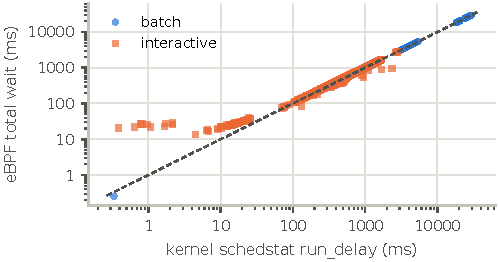
\includegraphics[width=\columnwidth]{figures/validation.pdf}
\caption{Per-thread eBPF wait vs.\ kernel \texttt{run\_delay} for all 2590 threads of the main grid (aggregate difference $-0.02\%$). The cluster at upper left consists of idle reference threads with a fixed 11--24\ms{} offset.}
\label{fig:validation}
\end{figure}

\begin{table}[t]
\centering
\footnotesize
\caption{Instrumentation overhead. Ratios are paired by seed with runs without the collector (median [95\% CI]); the maximum ring-buffer drop rate was 0.000\%.}
\label{tab:overhead}
\setlength{\tabcolsep}{3.5pt}
\begin{tabular}{@{}llrrrr@{}}
\toprule
& Collector & ns/ev. & CPU\,\% & Tput ratio & p99 ratio \\
\midrule
x1 & maps only & 514 & 0.025 & 0.99 {\scriptsize[0.96, 1.04]} & 1.03 {\scriptsize[0.85, 1.07]} \\
 & maps + events & 598 & 0.029 & 0.99 {\scriptsize[0.92, 1.02]} & 0.96 {\scriptsize[0.94, 1.19]} \\
x2 & maps only & 490 & 0.031 & 0.99 {\scriptsize[0.65, 1.01]} & 1.10 {\scriptsize[0.97, 1.61]} \\
 & maps + events & 565 & 0.035 & 0.99 {\scriptsize[0.98, 1.00]} & 1.09 {\scriptsize[1.02, 1.15]} \\
x4 & maps only & 485 & 0.031 & 0.99 {\scriptsize[0.63, 1.00]} & 1.01 {\scriptsize[0.96, 1.88]} \\
 & maps + events & 551 & 0.036 & 1.00 {\scriptsize[0.67, 1.00]} & 1.35 {\scriptsize[0.95, 1.77]} \\
\bottomrule
\end{tabular}
\end{table}


\subsection{H1: Unfairness Under EEVDF}\label{sec:h1}
Batch contention inflates interactive p99 by 1.7--2.2$\times$ for M1, 2.7--2.8$\times$ for M2 and 2.7--4.0$\times$ for M3 relative to running alone. SLO misses rise from 0.1\%, 0\% and 2.0\% to 1.5--2.9\%, 4.6--4.9\% and 14.5--20.4\% respectively. The damage comes in episodes, not uniformly. With batch work present, 20--35\% (M1), 83--87\% (M2) and 61--62\% (M3) of all 100\ms{} windows contain an SLO miss, against 1\%, 1\% and 30\% alone, and the longest episode lasts 3.1\,s (M2, x1). Fig.~\ref{fig:timeline} shows 61 of 300 windows missing the SLO in one M1 run while batch progress stays steady. The run-queue wait p99 of interactive threads grows from 27--394\us{} alone to 3.5--7.8\ms, one to three EEVDF base slices of 2.8\ms. By every long-run fairness measure the same runs look fair: Jain's index over normalized shares is at least 0.951, no batch thread ever goes a 100\ms{} window without progress, and the longest batch wait is 8--80\ms. The unfairness is \emph{temporal}, invisible to share metrics and visible to run-queue telemetry. H1 holds.

\begin{figure}[t]
\centering
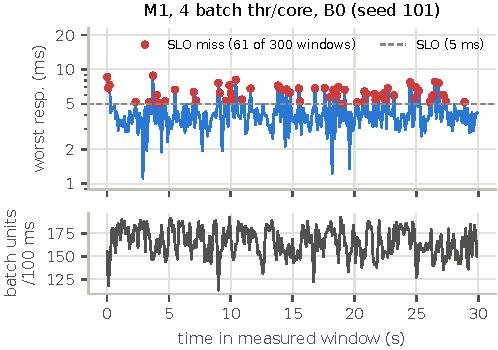
\includegraphics[width=\columnwidth]{figures/timeline_h1.pdf}
\caption{One B0 run (M1, x4). Top: worst response per 100\ms{} window; red dots miss the SLO. Bottom: batch work completed per window.}
\label{fig:timeline}
\end{figure}

\begin{figure*}[t]
\centering
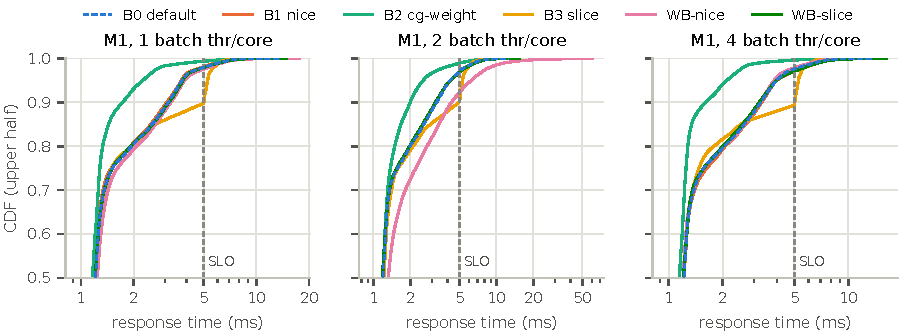
\includegraphics[width=\textwidth]{figures/cdf_M1.pdf}
\caption{Upper half of the M1 response-time distribution, all five seeds pooled. Only B2 (class weight) shifts the tail; B3's static slice adds a step at the SLO.}
\label{fig:cdf}
\end{figure*}

\begin{table*}[t]
\centering
\footnotesize
\caption{Every policy in every cell, relative to B0 (median of 5 seed pairs; All: the 45 main pairs pooled). \textbf{Bold}: the whole 95\% bootstrap CI is better than B0; {\normalfont\itshape italic}: the whole CI is worse. x$k$: $k$ batch threads per core.}
\label{tab:matrix}
\setlength{\tabcolsep}{4.2pt}
\begin{tabular}{@{}lrrrrrrrrrrrrr@{}}
\toprule
Policy & \multicolumn{3}{c}{M1} & \multicolumn{3}{c}{M2} & \multicolumn{3}{c}{M3} & \multicolumn{1}{c}{All} & \multicolumn{3}{c}{M4 (held out)} \\
\cmidrule(lr){2-4}\cmidrule(lr){5-7}\cmidrule(lr){8-10}\cmidrule(lr){12-14}
 & x1 & x2 & x4 & x1 & x2 & x4 & x1 & x2 & x4 & pairs & x1 & x2 & x4 \\
\midrule
B0 p99 (ms) & 6.0 & 6.4 & 5.7 & 4.3 & 4.3 & 4.3 & 8.7 & 10.3 & 11.9 &  & 25.3 & 28.5 & 27.2 \\
\addlinespace[2pt]\multicolumn{14}{@{}l}{\textit{Interactive p99 / B0}} \\
B1 nice & 0.93 & 0.97 & 0.98 & 0.99 & 1.02 & \textit{1.04} & 1.27 & 0.85 & 1.07 & 1.01 & 0.86 & 1.01 & \textit{1.20} \\
B2 cg-weight & \textbf{0.63} & \textbf{0.78} & \textbf{0.51} & \textbf{0.53} & \textbf{0.54} & \textbf{0.51} & \textbf{0.67} & \textbf{0.59} & \textbf{0.50} & \textbf{0.58} & \textbf{0.61} & \textbf{0.58} & \textbf{0.54} \\
B3 slice & 1.01 & 0.99 & 1.13 & 1.07 & 1.08 & 1.14 & 1.09 & 0.86 & \textit{1.30} & \textit{1.08} & 1.11 & 1.06 & 1.22 \\
WB-nice & 1.01 & \textit{1.14} & 1.11 & 0.99 & 0.99 & 0.99 & 1.05 & 1.03 & \textit{2.17} & \textit{1.03} & 1.17 & \textit{1.12} & \textit{1.51} \\
WB-slice & 1.02 & 1.01 & 1.02 & 0.95 & 0.98 & 1.05 & 0.91 & 1.09 & 1.38 & 1.01 & 1.05 & 1.07 & 1.01 \\
\addlinespace[2pt]\multicolumn{14}{@{}l}{\textit{Batch throughput / B0}} \\
B1 nice & 1.02 & 1.00 & 1.00 & 1.01 & 1.00 & 0.99 & 1.01 & 1.01 & 1.01 & 1.00 & 1.01 & 0.99 & 0.99 \\
B2 cg-weight & 0.99 & 1.00 & 1.00 & 1.00 & 1.00 & 0.99 & 1.00 & 0.99 & 0.98 & 1.00 & 1.01 & \textit{0.98} & 0.99 \\
B3 slice & 1.00 & 1.01 & 1.01 & 1.01 & 1.01 & 1.00 & 0.99 & 1.00 & 1.01 & 1.01 & \textbf{1.02} & 1.00 & 1.01 \\
WB-nice & 0.98 & \textit{0.93} & 1.00 & 1.00 & 1.02 & 1.00 & 1.01 & 1.00 & 0.99 & 1.00 & 1.02 & 1.00 & 0.99 \\
WB-slice & 0.99 & 1.00 & 1.00 & 1.04 & 1.02 & 1.00 & 1.02 & 1.01 & 1.00 & 1.00 & 1.00 & 0.99 & \textit{0.98} \\
\bottomrule
\end{tabular}
\end{table*}


\subsection{Mitigation: Only Class Weight Works}\label{sec:mitigation}
Table~\ref{tab:matrix} compares every policy with B0. Static class weight (B2) cuts interactive p99 by 22--50\% in all nine main cells and by 39--46\% on the held-out M4. Every confidence interval lies below 1, and all 45 pooled main pairs improve (median ratio 0.58, Wilcoxon $p=6\times10^{-14}$). SLO misses fall by 61--85\% (Fig.~\ref{fig:cdf}), while batch throughput stays within 2\% of B0 in every cell. No per-task policy helps. Static nice (B1) has a pooled ratio of 1.01 ($p=0.65$). The static short slice (B3) makes p99 8\% \emph{worse} ($p=0.017$). WaitBoost with either per-task actuator changes p99 by $+1\%$ (slice) and $+3\%$ (nice), with its worst cell at $2.2\times$ (M3, x4). WaitBoost did act, with a median of 35--97 boosts per run and no guard activations, actuator errors or failed restores.

The cause is the cgroup hierarchy. With group scheduling, every cgroup has its own run queue, and at the parent level each cgroup is represented by a single scheduling entity whose weight is its \cpuweight~\cite{kernel-cgroupv2}. A thread's nice value sets its weight only relative to its siblings in the same cgroup. B1 lowers every batch thread equally, which leaves both the threads' relative weights and the batch group's weight unchanged, so it is a no-op by construction. WB-nice raises one interactive thread above other interactive threads, not above batch work. A custom slice likewise reorders a thread among its siblings, while the interactive group still competes with the batch group at equal weight. A slice shorter than the request also splits it: under B3, 8.6--9.3\% of interactive switches are involuntary (1.0--1.7\% under B0), and each preempted fragment may queue behind a batch slice, which produces the step at the SLO in Fig.~\ref{fig:cdf}. WB-slice avoids the splitting through its burst floor (1.3--2.2\% involuntary) but still gains nothing. Class weight acts where the two classes actually compete, and because the interactive class is demand-limited, a 4:1 weight lets it run sooner without changing long-run shares. Fig.~\ref{fig:waits} shows the interactive wait p99 falling from 4.0 to 1.5\ms{} in M1 at x4 while the longest batch wait does not grow. In 5 of 12 cells B2 does lengthen the longest batch wait, by up to 1.6$\times$ (M4, x1: 16 to 26\ms), but it never exceeds 76\ms{} and no starved window occurs. H2 therefore holds only for class-level actuation. H3 is rejected: the slice actuator neither matched the benefit of weight nor improved on B0.

\begin{figure}[t]
\centering
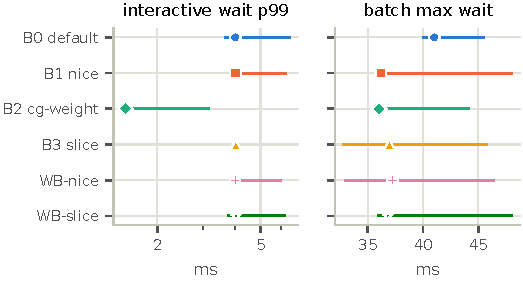
\includegraphics[width=\columnwidth]{figures/waits_M1_x4.pdf}
\caption{Run-queue waits in M1 at x4: interactive p99 and the longest batch wait (median and 95\% CI over seeds).}
\label{fig:waits}
\end{figure}

\subsection{Ablations and Sensitivity}
Table~\ref{tab:ablation} confirms the diagnosis. Removing aging or wait feedback from the per-task variants changes nothing, because the knob they move is inert. Driving the class weight from the measured wait (WB-cg) helps: p99 falls by 14\% [8, 31] with all 15 pairs improving, and by 37\% in the bursty M3, at no throughput cost. WB-cg still trails static B2 because it reacts only after waits have built up, whereas B2 gives preference from the first wake-up. Its value is that the boost is bounded, decays and is dropped by the starvation guard, protections a static weight lacks if a latency-sensitive class turns CPU-hungry. Fig.~\ref{fig:theta} shows that no threshold between 0.25 and 4\ms{} makes WB-slice useful. It also calibrates our noise. The tuned policy and the sweep point at $\theta=2$\ms{} are the same configuration run separately, and they differ by up to 7\%, so effects below about 10\% at five seeds should be read as noise. On the held-out M4 the per-task policies range from 0.86 to 1.51$\times$ B0, with no interval entirely below 1 (Table~\ref{tab:matrix}). Across 1--3 experiment cores they stay within 0.96--1.07$\times$ B0, while B0's own p99 falls from 8.5 to 5.6\ms.

\begin{table}[t]
\centering
\footnotesize
\caption{Ablations at 2 batch threads per core, pooled over M1--M3 (15 seed pairs per row; marks as in Table~\ref{tab:matrix}). Boosts: median boost actions per run.}
\label{tab:ablation}
\setlength{\tabcolsep}{4pt}
\begin{tabular}{@{}lrrrr@{}}
\toprule
Variant & p99/B0 [95\% CI] & Tput & Max wait & Boosts \\
\midrule
WB-nice & \textit{1.04} {\scriptsize[1.01, 1.07]} & 1.00 & 1.00 & 73 \\
\quad no aging & 1.01 {\scriptsize[0.99, 1.05]} & 1.00 & 0.95 & 20 \\
\quad no wait feedback & 1.00 {\scriptsize[0.96, 1.08]} & 1.00 & 1.00 & 5 \\
WB-slice & \textit{1.03} {\scriptsize[1.01, 1.06]} & \textbf{1.01} & 0.96 & 83 \\
\quad no aging & 1.03 {\scriptsize[0.97, 1.07]} & 1.00 & 0.98 & 20 \\
\quad no wait feedback & 1.04 {\scriptsize[0.98, 1.09]} & 1.00 & \textbf{0.87} & 5 \\
WB-cg (per class) & \textbf{0.86} {\scriptsize[0.69, 0.92]} & 1.00 & 0.93 & 243 \\
\bottomrule
\end{tabular}
\end{table}


\begin{figure}[t]
\centering
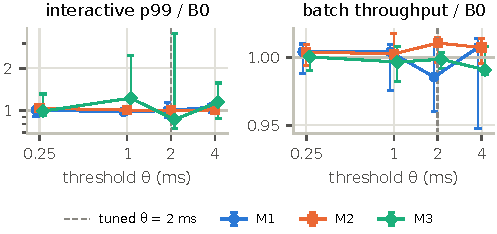
\includegraphics[width=\columnwidth]{figures/theta_sweep.pdf}
\caption{WB-slice threshold sweep at x2 (median and 95\% CI of seed pairs; the p99 axis is logarithmic).}
\label{fig:theta}
\end{figure}

% ===================================================================================== V
\section{Conclusion}
EEVDF keeps long-run CPU shares fair but lets batch contention inflate interactive p99 by up to 4$\times$ in episodes lasting seconds, which only per-thread run-queue telemetry reveals. The mitigation result is a practical warning: when interactive and batch work live in different cgroups, as under systemd and container runtimes, nice values and EEVDF custom slices cannot move CPU time between them, and boosting those knobs, however carefully bounded, accomplishes nothing. Class-level \cpuweight{} does, with no measurable throughput cost while the latency-sensitive class is demand-limited, and WaitBoost on that knob adds bounded, self-revoking control. \textit{Limitations}: all runs used one laptop under WSL2, whose 0.48\ms{} p99 wake-up lag sets a floor on absolute latency, and one kernel version. Five seeds per cell resolve only effects of roughly 10\% or more. The workloads are synthetic spin loops, and the scaling runs did not include B2. Future work should test an adversarial, CPU-hungry interactive class, where WaitBoost's guard and revocation matter, and port the policy to \texttt{sched\_ext}, where it could act within the hierarchy rather than across it.

\bibliographystyle{IEEEtran}
\bibliography{refs}

\end{document}
